
\documentclass{beamer}
\usetheme{Madrid}
\documentclass[12pt]{article}
\usepackage[utf8]{inputenc}
\usepackage{physics}
\usepackage[margin=1in]{geometry}
\usepackage{graphicx}
\usepackage[english]{babel}
\usepackage{mathabx}
\usepackage{mathptmx}
\usepackage{dsfont}
\usepackage{amsmath}
\usepackage{caption, threeparttable}
\captionsetup{labelfont = sc, textfont = it}
\title{Investigating Ferromagnetic Alloys for JMRAM Spintronic Transistors}
% A subtitle is optional and this may be deleted

\subtitle{via self-consistent computational methods}
\author{Nikolaos Palamidas}
\institute[] % (optional, but mostly needed)
{
  \inst{}%
  Department of Physics\\
  King's College London
 }
\date{27th March, 2017}
\begin{document}
\begin{frame}
  \titlepage
\end{frame}
\begin{frame}{Outline}
  \tableofcontents
  % You might wish to add the option [pausesections]
\end{frame}

\section{The JMRAM}

\begin{frame}{JMRAM}{Tunnel Magnetoresistance}
  \begin{itemize}
  \item {Josephson Effect leads to Cooper pair rotation}
  \item {Supercurrent experiences high or low resistance from relative magnetisation.}
  \item{Tunnel Magnetoresistance}
  \end{itemize}
 \begin{figure}[h!]
    \centering
    \begin{measuredfigure}
    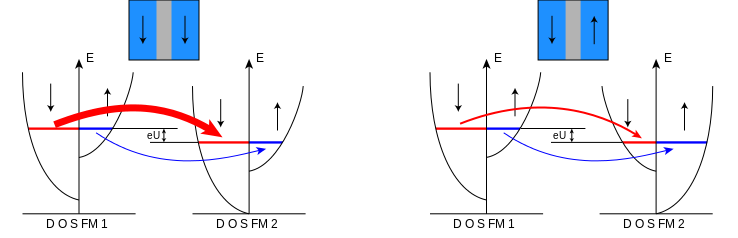
\includegraphics[scale=0.4]{tmr}
    \caption{https://en.wikipedia.org/wiki/Tunnel\_magnetoresistance}
    \end{measuredfigure}
    \end{figure}
\end{frame}
\begin{frame}{JMRAM}{Anatomy of a magnetic tunneling junction}
  \begin{itemize}
      \item {High or low current corresponds to logic bit states.}
      \item{Free layer must be able to switch quickly and efficiently.}
      \item{Must have low magnetisation, low magnetostriction, and low scattering.}
  \end{itemize}
  \begin{figure}[h!]
    \centering
    \begin{measuredfigure}
    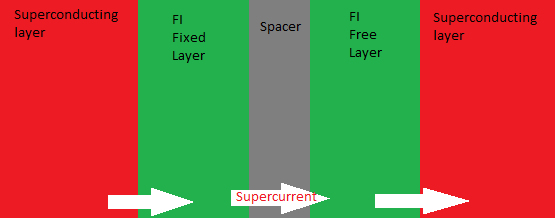
\includegraphics[scale=0.7]{mtj}
    \end{measuredfigure}
    \end{figure}
\end{frame}
\begin{frame}{JMRAM}{Electron pair transport}
\begin{itemize}
    \item {Cooper pairs of electrons in superconductor form in opposite spin and momentum states(according to BCS theory).}
    \item{Cooper pairs in a ferromagnetic local environment will break due to Lorentz force.}
    \item{To survive, the pair must "rotate".}
    \item{Josephson effect predicts a phase difference in the wavefunction in the ferromagnetic layer.}
    \item{$\Psi=\frac{1}{\sqrt{2}}[e^{i\theta}\ket{\updownarrows}_{k,-k}- e^{-i\theta}\ket{\downuparrows}_{k,-k}]$\cite{contact}}
    \item{Layers must be thin as tunneling is not deep.}
\end{itemize}
\end{frame}

\section{Density Functional Theory}

\begin{frame}{Self-Consistent Computational Methods}{Hohenberg-Kohn Theorems}
  \begin{itemize}
      \item {The energy of a many body can always be expressed as a unique functional of the density $E[n(r)]$(very easy to prove).}
      \item{By variation of the density $n(r)$, one can obtain the minimum global energy, which is the ground state energy $E_0=E[n_0(r)]$}
      \item{Forms the basis of density functional theory.}
  \end{itemize}
\end{frame}
\begin{frame}{Self-Consistent Computational Methods}{Density Functional Theory}
  \begin{itemize}
        \item {Real system acts in $V_{ext}(r)$. Make an auxiliary $V_{eff}(r)$}
        \item{$E[n]=\int V\textsubscript{ext}(r)n(r)d^3r + T[n] + V_\textsubscript{ee}[n]$}
      \item{All electron-electron interaction $V_{ee}$ a combination of the Hartree potential and an unknown contribution $\xi(r)$}
      \item{Kohn-Sham equation $H_s \psi_i (r) = (-\frac{\hbar^2}{2m}\nabla^2 +V_e_f_f(r) ) \psi_i (r)=T_s[n]+V_{eff}[n]$}
      \item{$E[n]_{total}=T[n]+V_e_e[n] = T_s[n] + \frac{1}{2}\int \int \frac{n(r)n(r')}{|r-r'|}d^3 r' + E_X_C[n]$}
      \item{Obtain $E_X_C[n]=T[n] -T_s[n] + \xi_{ee}[n]$  }
      \item{Can be approximated by the Local density approximation (Homogeneous electron gas/Jellium)}
  \end{itemize}
\end{frame}
\begin{frame}{Self-Consistent Computational Methods}{Iterative procedure}
    \begin{itemize}
    \item{Guess an input $n_{in}$ and obtain the corresponding effective potential $V_{in}$, and use Kohn-Sham to find $\Psi_{in}$.}
\item{Input $\Psi$ gives an output density}
\item{If not the input density, iterate.}
\end{itemize}
\end{frame}

\section{Linear Muffin Tin Orbitals}

\begin{frame}{Appropriate basis set}{MTOs}
  \begin{itemize}
      \item {LMTO basis is appropriate basis for describing electrons in metals.}
      \item{Spherical potential around nuclei site and flat potential in the interstitial.}
      \item{Solve Schrodinger in site, and Laplace in the interstitial.}
      \item{Solution to the 3D Schrodinger equation is Hankel and Bessel functions}
      \item{Regular $J_l(r)$ and Irregular $K_l(r)$ solutions.}
      \item{Linear combination of J and K, must solve all space.}
      \item{By Wronskian method we ensure that the radial $\phi_l(r)$ matches smoothly and differentiably onto some $A\cdot J_l+B\cdot K_l$.}
  \end{itemize}
\end{frame}
\begin{frame}{MTOs}{Single site solution}
  \begin{itemize}
      \item {at the sphere boundary we have the condition that $N_R_l \varphi_R_l= K_l(r)- P_R_l(E) J_l(r) \quad r=s$}
      \item{$\Psi_R_l(r,E)=N_R_l &(E)\varphi_R_l(r,E) +P_R_l(E)J_l(r_R) \qquad r<s_R \qquad HEAD$}
      \item{$\Psi_R_l(r,E)=K_l(E) \qquad r>s_R \qquad TAIL$}
      \item{Only for a single site. True wavefunction is linear combination of each site contribution}
  \end{itemize}
\end{frame}
\begin{frame}{MTOs}{Multiple site solution}
  \begin{itemize}
      \item {Each site solution TAIL trespasses or leaks into other sites}
      \item{One can write irregular solution K as a combination of regular solution J centred at other sites.}
      \item{$K_l(r)=-\sum_{L'} S_{RL,R'L'} J_{L'}(r_{R'})$}
      \item{To maintain true Schrodinger solution, must ensure that J contributions in each site cancel(tail cancellation).}
      \item{Use matrices of RL by R'L'}
      \item{$det[P_{Rl}(E)\delta_{RL,R'L'}-S_{RL,R'L'}]$}
      \item{Alternative matrix notation $|(P-S)|=0$}
  \end{itemize}
\end{frame}
\begin{frame}{Energy Linearisation}
    \begin{itemize}
        \item{Choose $E_\nu$ such that wavefunctions are energy-independant}
        \item{Taylor expansion $\varphi(r,E) = \varphi_{\nu} + \dot{\varphi}_{\nu}(E-E_\nu)+O(E-E_\nu)^2=\phi + \dot{\phi}(E-E_\nu)+O(E-E_\nu)^2$}
        \item{$\dot{\phi}$ and $\phi$ are able to describe smooth functions }
        \item{Describe the envelope function $K_l(r)$ and augment inside the sphere to describe MTOs.}
        \item{Wronskians for matching K onto linear combination of $\dot{\phi}$ and $\phi$}
        \item{Only in first order of $E-E_\nu$ so does not solve Schrodinger exactly.}
    \end{itemize}
\end{frame}

\begin{frame}{LMTO basis}{Hamiltonian and Orthogonal matrix}
    \begin{itemize}
        \item {If energy linearised $H_{ij}-E_\nu O_{ij}=0$}
        \item{$H^{orth}_{RL,R'L'}=C_{RL}\delta_{RR'}\delta_{LL'} + \sqrt{\Delta_{RL}}S_{RL,R'L'}(1-\gamma_{RL} S_{RL,R'L'})^{-1} \sqrt{\Delta_{R'L'}}$}
        \item{In this rep $O^{orth}_{RL,R'L'}=\delta_{RR'}\delta_{LL'}$}
        \item{}
        \item{}
    \end{itemize}
\end{frame}

\begin{frame}{Green's Functions}{Multiple Scattering theory}
    \begin{itemize}
        \item {MST describes the propagation of a wave through multiple scatterers (Korringa). Along with DFT (Kohn) forms KKR method.}
        \item{Green's function able to solve otherwise analytically impossible equations.}
        \item{Green's function has ability to be averaged(CPA).}
        \item{$G(E)=(E\mathds{1}-H^{orth})^{-1}$}
        \item{Propagation of wavefunction described by $\psi(x,t)=\int dy G(x,t,y,t')\psi(y,t')$}
    \end{itemize}
\end{frame}

\begin{frame}{Green's Functions}{Perturbations}
    \begin{itemize}
        \item {Free/bare Green's function $G^0$ and perturbed(real) G}
        \item{Perturb Hamiltonian by some potential V $H=H^0+V$.}
        \item{$G(E)=(E-H)^{-1}$ and $G^0(E)=(E-H^0)^{-1}$}
        \item{Leads to Born expansion $G(E)=G^0+G^0VG=G^0+G^0VG+G^0VG^0VG^0+...$}
        \item{$G(E)=G^0+G^0(V+VG^0V+...)G^0=G^0+G^0T(E)G^0$ T-matrix related to scattering}
        \item{$T(E)=[1-VG^0]^{-1}V$ becomes important for CPA.}
    \end{itemize}
\end{frame}

\begin{frame}{LMTO GF}
    \begin{itemize}
        \item {$G^{orth}_{RL,R'L'}(E)=\Delta^{-1/2}(P-S)^{-1}\Delta^{-1/2}$ Matrix form.}
        \item{$(P-S)^{-1}$ solves Tail-cancellation and is valid Green's function solution.}
        \item{Define Auxiliary Green's Function.}
        \item{Easier to obtain computationally, and used for CPA.}
        \item{Recall $g(E)=(P-S)^{-1}$}
    \end{itemize}
\end{frame}
\section{CPA theory}
\begin{frame}{Coherent Potential Approximation}{Configurational average}
    \begin{itemize}
        \item{Need way to model random alloys}
        \item{Replace system by effective medium of no fluctuations.}
        \item{$c^A+c^B=1$ and so $<G_{RR}(E)>= \sum_Q c_R^Q <G_{RR}^Q(E)>$}
        \item{Recall $g(E)=(P-S)^{-1}$}
        \item{Replace P with a energy dependant constant function $\mathcal{P}$ to describe the configurational average. }
        \item{$\expval{g_{RL,R'L'}(E)}=[\mathcal{P}(E)-S]^{-1}_{RL,R'L'}$}
        
    \end{itemize}
\end{frame}

\begin{frame}{CPA}{The effective medium}
    \begin{itemize}
        \item{Focus on a central site, endowed with $c^Q$, all other sites expressed via coherent potential.}
        \item{Impose that no extra average scattering upon addition of Q type atom into $\matchal{P}$. i.e. $\sum_Qc_R^Qt_R^Q(E)=0$}
        \item{$T(E)=\sum_it_i(E)$ assuming no overlap.}
        \item{Perturbation is full potential and bare/coherent difference; $\Delta^Q_R=P_R^Q-\mathcal{P}^Q_R$}
        \item{$t_R^Q(E)=\Delta^Q_R\bigg[1+\expval{g_{RR}}(E)\Delta^Q_R\bigg]^{-1}$}
    \end{itemize}
\end{frame}
\section{The Magnetic Tunneling Junction}
\begin{frame}{Material Properties}
  \begin{itemize}
      \item {For TMR, we must have a ferromagnetic insulating material.}
      \item {Low Magnetostriction (origins in anisotropy)}
      \item {Low magnetic moment/magnetisation}
      \item {Low scattering/high spin lifetime}
      \item {Low scattering at superconductor-ferromagnetic interface.}
  \end{itemize}
\end{frame}

\begin{frame}{MTJ}{Possible alloy choice}
  \begin{itemize}
      \item {It has been proposed that the alloy of choice be Permalloy, typically $Fe_{20}Ni_{80}$.}
      \item {Magnetic moment too high, so alloyed with copper.}
      \item {Attempt at trying Fe-Cr alloy to see the difference.}
      \item {Superconductor choice must have reasonable transition temperature(e.g. Pb/Nb).}
      \item {Choose alloy with similar crystal structure and lattice constant to superconductor so that band levels line up.}
  \end{itemize}
\end{frame}

\begin{frame}{Obtaining results}{Observables from GF}
  \begin{itemize}
      \item { $\lim_{\eta\to\ 0^+}Im[\frac{1}{E+i\eta-\epsilon_i}]=\lim_{\eta\to\ 0^+}(-\frac{\eta}{(E-\epsilon_i)^2-\eta^2})=-i\pi \delta(E-\epsilon_i)$}
      \item {$\lim_{\eta\to\ 0^+}Im[-\frac{1}{\pi}G(r,r',E-\epsilon_i)]=\sum_i \psi^*_i\psi_i \delta(E-\epsilon_i)=\omega(E,r)$ Energy-resolved density.}
      \item {$n(r)=\int_{-\infty}^{E_F}\omega(E,r) \qquad D_{3D}(E)=\int \omega(E,r) d^3r$}
      \item {Or one can take the Fourier-transformed Green's function $G(k,\omega)$, and follow a similar prescription.}
      \item {$\mathcal{A}(k,E)=-\frac{1}{\pi} Im[\sum_L G(k,E+i0^+)_L_L]$ Bloch Spectral Function.}
      \item{In CPA case G replaced with $\expval{G}$.}
  \end{itemize}
\end{frame}

\begin{frame}{QUESTAAL suite}{lmgf}
  \begin{itemize}
      \item {'lmgf' is a Green's function code that employs LMTO-ASA theory with self-consistent spin DFT in the LSDA. CPA can also be incorporated for random alloys.}
      \item {Outputs magnetisation,exchange integrals, and can produce spectral functions.}
      \item {}
      \item {}
      \item {}
  \end{itemize}
\end{frame}

\begin{frame}{Permalloy-Copper alloy}{Curie Temperature}
      \begin{table}[h!]
\centering
 \begin{tabular}{||c c c c c c||} 
 \hline
 Alloy Ratio & $J_0^{Fe}$ & $J_0^{Ni}$ & $J_0^{Cu}$ & $J_0^{Total}$ & Curie $T_C$ \\ [1ex] 
 \hline\hline
 $Py$ & 10.34 & 4.607 & null & 5.7536 & 605.38 \\ 
 $Py_{80}Cu_{20}$ & 8.662 & 2.509 & 0.096 & 3.01088 & 316.80 \\
 $Py_{60}Cu_{40}$ & 6.731 & 1.861 & 0.056 & 1.7234 & 181.33 \\
 $Py_{40}Cu_{60}$ & 5.297 & 1.148 & 0.022 & 0.80432 & 84.63 \\
 $Py_{20}Cu_{80}$ & 2.447 & 0.052 & 0.003 & 0.1086 & 11.43 \\ [1ex] 
 \hline
 \end{tabular}
\caption{The calculation of Curie temperature T\textsubscript{C}(K) from exchange constants J\textsubscript{0}(mRy), for different ratios of pure permalloy Py-$Fe_{20}Cr_{80}$ and copper Cu.} 
\end{table}
\end{frame}

\begin{frame}{Permalloy-Copper Alloy}{Magnetisation}
\begin{table}[h!]
\centering
 \begin{tabular}{||c c||} 
 \hline
 Alloy Ratio & Magnetisation[$emu/cm^3$] \\ [1ex] 
 \hline\hline
 $Py$ & 1144.67 \\ 
 $Py_{80}Cu_{20}$ & 615.49 \\
 $Py_{60}Cu_{40}$ & 445.70 \\
 $Py_{40}Cu_{60}$ & 277.08 \\
 $Py_{20}Cu_{80}$ & 89.76 \\ [1ex] 
 \hline
 \end{tabular}
\caption{The calculation magnetic moment for different ratios of pure permalloy Py-$Fe_{20}Ni_{80}$ and copper Cu, in units of $[emu/cm^3]$.} 
\end{table}
\end{frame}

\begin{frame}{Permalloy-Copper Alloy}{Spectral Functions}
 \begin{figure}[htp]
    \centering
    \begin{measuredfigure}
    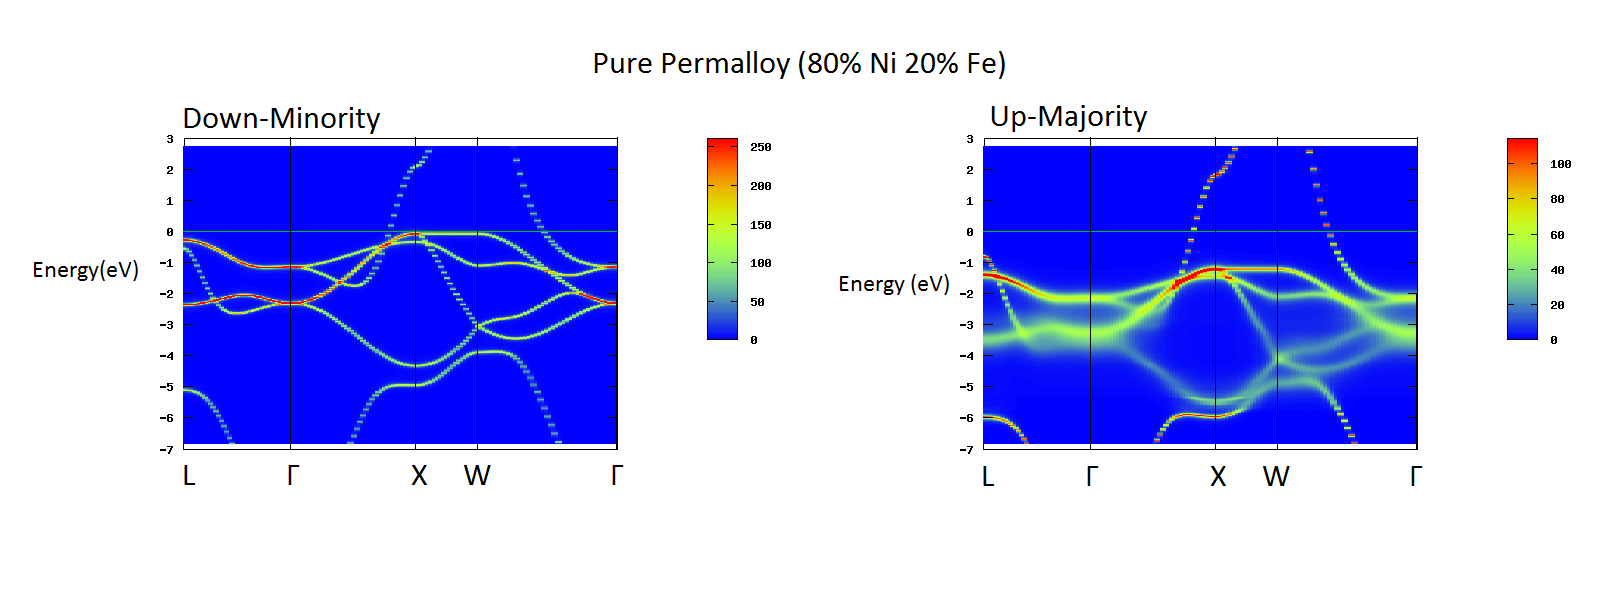
\includegraphics[scale=0.27]{purepy}
    \caption{Plotted Bloch Spectral function for pure Permalloy $Py=Fe_{20}Ni_{80}$ via lmgf calculations.}
    \end{measuredfigure}
    \end{figure}
\end{frame}
\begin{frame}{Permalloy-Copper Alloy}{Spectral Functions}
  \begin{figure}[h!]
    \centering
    \begin{measuredfigure}
    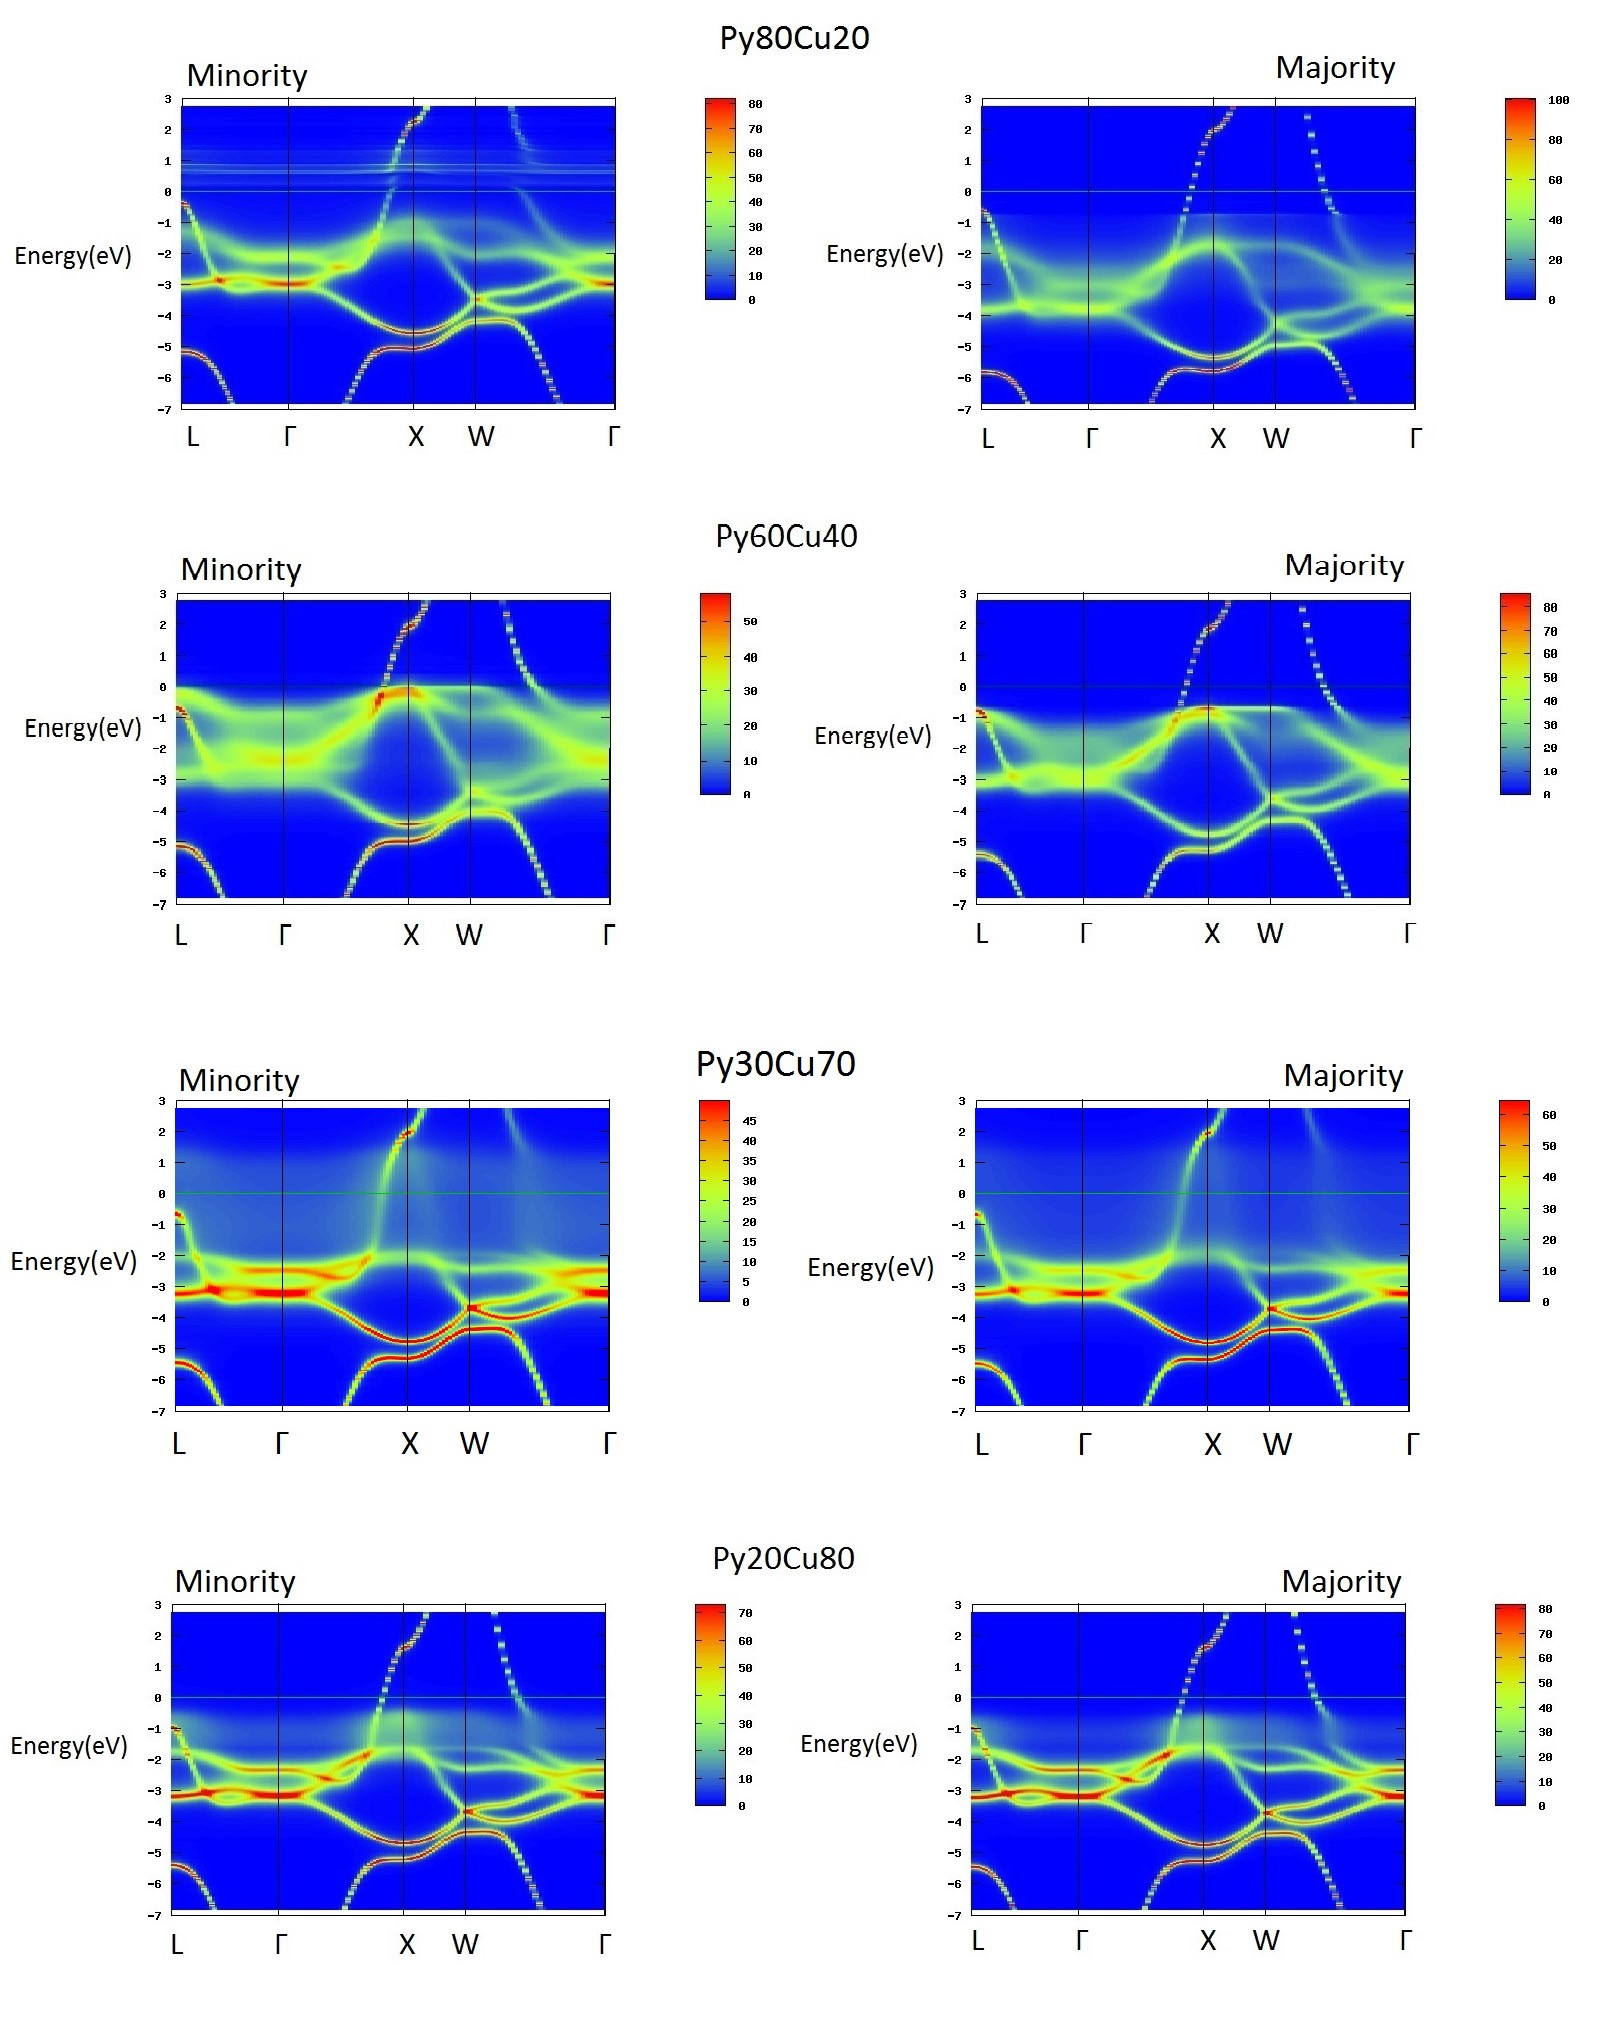
\includegraphics[scale=0.14]{py}
    \end{measuredfigure}
    \end{figure}
\end{frame}
\begin{frame}
  \begin{itemize}
      \item {The ideal alloy is that which balances low magnetisation and low scattering.}
      \item{Perhaps there exists a 'perfect' alloy configuration to balance all properties.}
      \item{Retain Iron, but replace nickel with chromium. See if pure FeCr is good.}
      \item{Alloy with copper if needed.}
  \end{itemize}
\end{frame}
\begin{frame}{Iron-Chromium Alloy}{Spectral functions}
\begin{figure}[h!]
    \centering
    \begin{measuredfigure}
    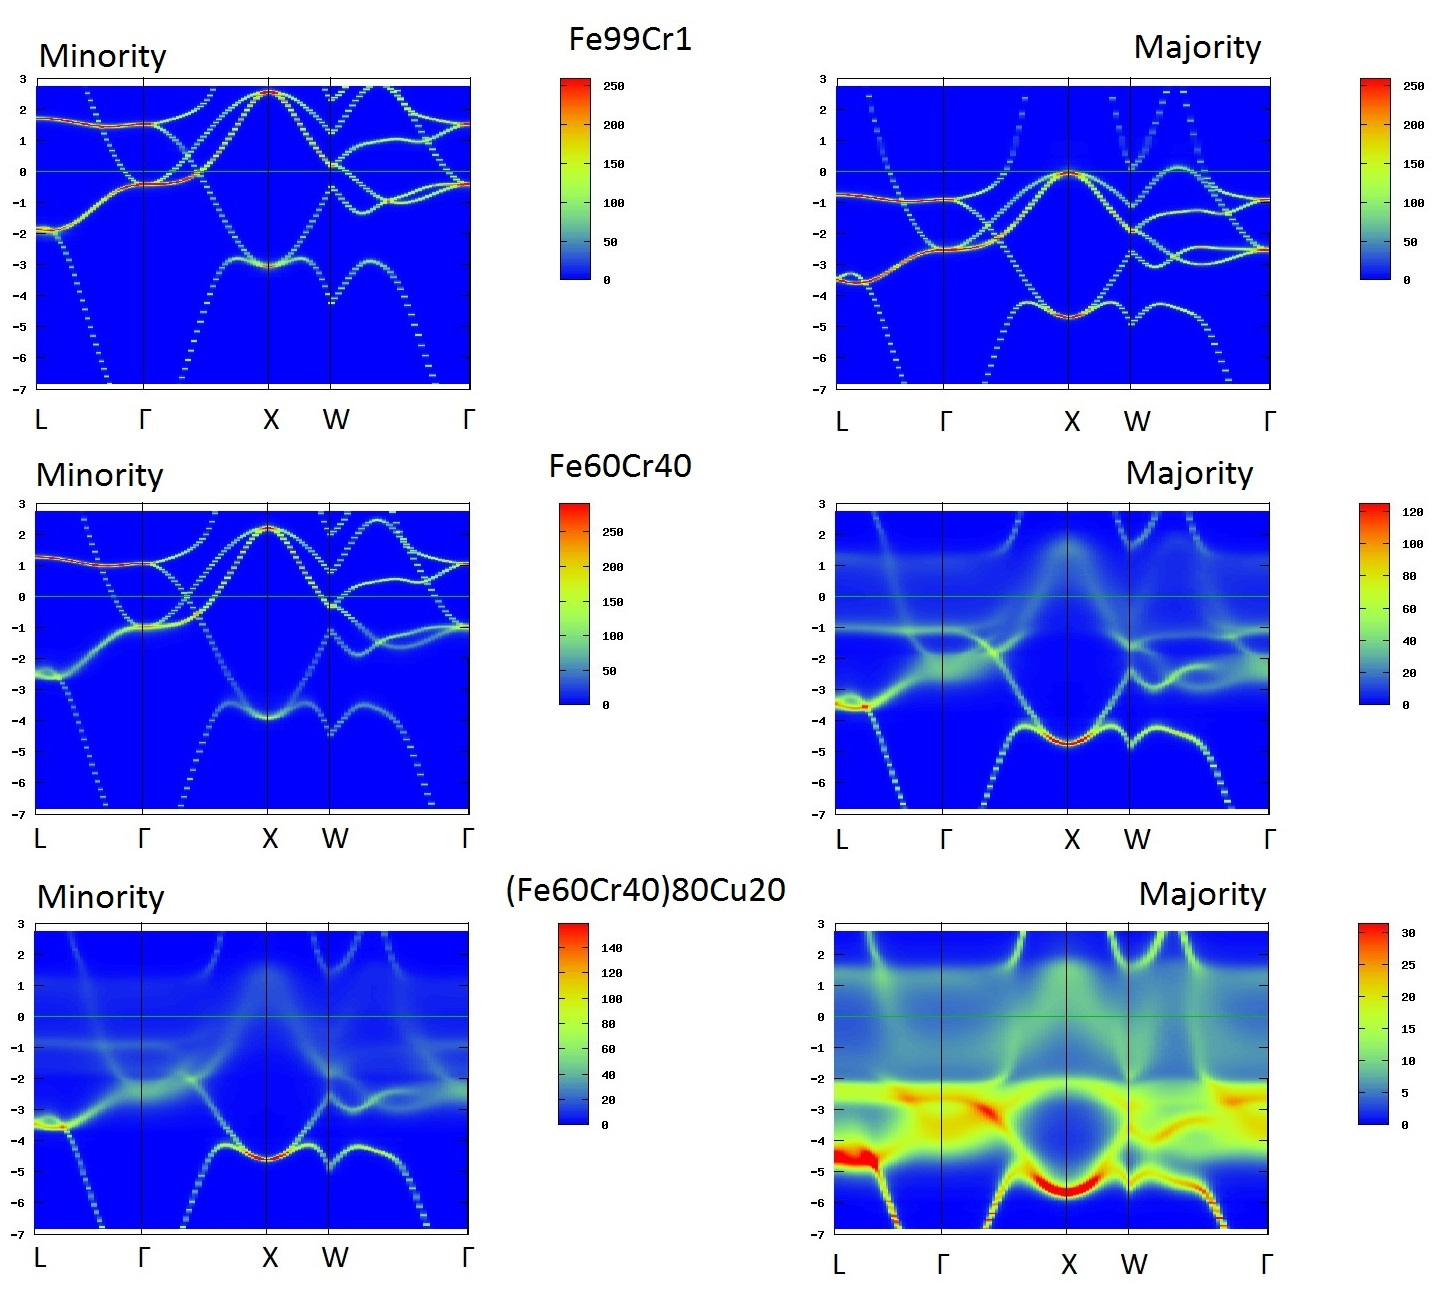
\includegraphics[scale=0.20]{Fe60Cr40}
    \end{measuredfigure}
    \end{figure}
\end{frame}
\begin{frame}{Iron-Chromium Alloy}{Spectral functions}
 \begin{figure}[h!]
    \centering
    \begin{measuredfigure}
    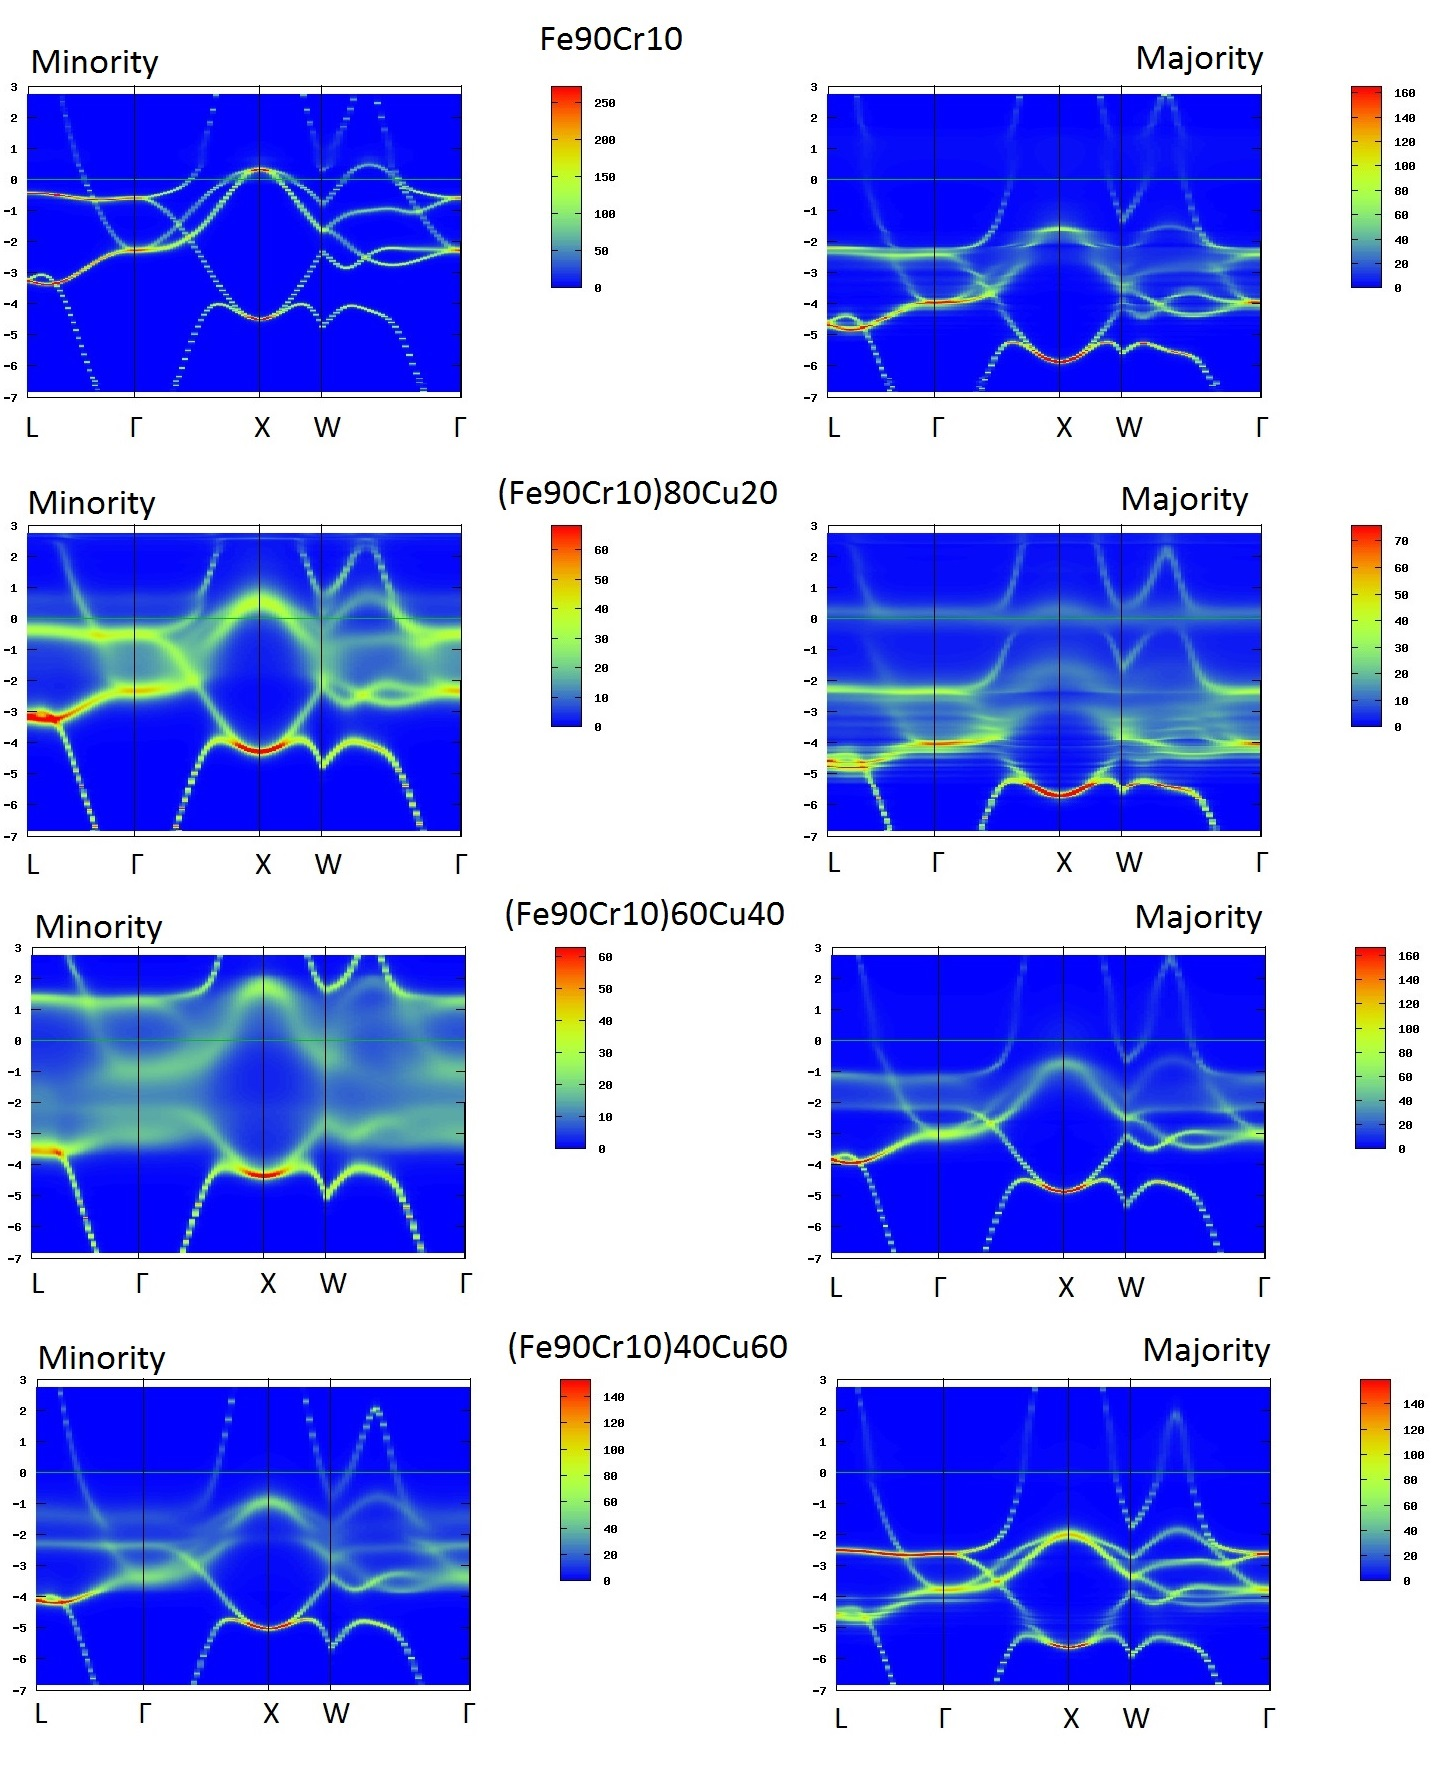
\includegraphics[scale=0.16]{Fe90Cr10}
    \end{measuredfigure}
    \end{figure}
\end{frame}
\begin{frame}{Iron-Chromium Alloy}{Magnetisation}
  \begin{table}[h!]
\centering
 \begin{tabular}{||c c||} 
 \hline
 Alloy Ratio & Magnetisation[$emu/cm^3$] \\ [1ex] 
 \hline\hline
 $Fe_{99}Cr_1$ & 1893.10\\ 
 $Fe_{90}Cr_{10}$ & 1627.15\\
 $Fe_{60}Cr_{40}$ & 964.56 \\
 $(Fe_{90}Cr_{10})_{90}Cu_{20}$ & 1316.01\\ 
 $(Fe_{90}Cr_{10})_{60}Cu_{40}$ & 1007.13\\  
 $(Fe_{90}Cr_{10})_{40}Cu_{60}$ & 664.71\\
 $(Fe_{60}Cr_{40})_{80}Cu_{20}$ & 774.99\\ [1ex]
 \hline
 \end{tabular}
\caption{The calculation magnetic moment for different ratios of pure permalloy Py-$Fe_{x}Cr_{1-x}$, in units of $[emu/cm^3]$.} 
\end{table}
\end{frame}
\begin{frame}{Iron-Chromium Alloy}{Curie Temperature}
  \begin{table}[h!]
\centering
 \begin{tabular}{||c c c c c c||} 
 \hline
 Alloy Ratio & $J_0^{Fe}$ & $J_0^{Cr}$ & $J_0^{Cu}$ & $J_0^{Total}$ & Curie $T_C$ \\ [1ex] 
 \hline\hline
 $Fe_{99}Cr_1$ & 12.369 & 15.346 & null & 12.399 & 1304.58 \\ 
 $Fe_{90}Cr_{10}$ & 12.358 & 6.98 & null & 11.820 & 1243.702\\
 $Fe_{60}Cr_{40}$ & 9.238 & 0.457 & null & 5.726 & 602.438 \\
 $(Fe_{90}Cr_{10})_{90}Cu_{20}$ & 11.020 & 7.487 & 0.046 & 8.543 & 898.834 \\ 
 $(Fe_{90}Cr_{10})_{60}Cu_{40}$ & 10.337 & 6.238 & 0.068 & 5.983 & 629.570 \\
 $(Fe_{90}Cr_{10})_{40}Cu_{60}$ & 8.835 & 3.518 & 0.077 & 3.368 & 354.325 \\ 
 $(Fe_{60}Cr_{40})_{80}Cu_{20}$ & 7.330 & 0.524 & 0.019 & 3.690 & 388.243 \\
 $(Fe_{60}Cr_{40})_{60}Cu_{40}$ & 6.015 & 0.553 & 0.029 & 2.310 & 243.025 \\ [1ex]
 \hline
 \end{tabular}
\caption{The calculation of Curie temperature T\textsubscript{C}(K) from exchange constants J\textsubscript{0}(mRy), for different ratios of Iron-chromium alloy, and alloyed with copper Cu.} 
\end{table}
\end{frame}
\begin{frame}{Conclusions}{Interpreting the results}
  \begin{itemize}
      \item {}
  \end{itemize}
\end{frame}





\appendix
\section<presentation>*{\appendixname}
\subsection<presentation>*{For Further Reading}

\begin{frame}[allowframebreaks]
  \frametitle<presentation>{For Further Reading}
    
  \begin{thebibliography}{10}
    
  \beamertemplatebookbibitems
  % Start with overview books.

  \bibitem{Author1990}
    A.~Author.
    \newblock {\em Handbook of Everything}.
    \newblock Some Press, 1990.
 
    
  \beamertemplatearticlebibitems
  % Followed by interesting articles. Keep the list short. 

  \bibitem{Someone2000}
    S.~Someone.
    \newblock On this and that.
    \newblock {\em Journal of This and That}, 2(1):50--100,
    2000.
  \end{thebibliography}
\end{frame}

\end{document}


